\documentclass[a4paper,11pt,pdf]{pacmanreport}

%%=== Aditional packages
\usepackage{amsmath}
\usepackage{amsfonts}

% The following is used to make packages hyperref and cite work together
\makeatletter
\let\NAT@parse\undefined
\makeatother
\usepackage[bookmarks=true,hyperfootnotes=true,colorlinks=true,linkcolor=blue,anchorcolor=blue,citecolor=blue,urlcolor=blue,filecolor=blue]{hyperref}

%%=== Local definitions
\graphicspath{{images/}{../shared_images/}}

%% ================================
%% PROJECT INFO

\project{}
\projectid{FP7-IST-60918}
\projectstart{1 March 2013}
\duration{36}

%% ================================
%% DELIVERABLE INFO

\title{Methodologies for grasp acquisition and planning}
\deliverableid{DR 4.3}
\author{H. Marino, C.J.~Rosales, M. Kopicki, G. Santaera, E. Luberto, Y. Wu, A. Artoni, G. Pannocchia, M. Gabiccini, and J.L.~Wyatt}
\address{University of Birmingham, UK}
\email{jlw@cs.bham.ac.uk}
\headertitle{Grasp acquisition and planning}
\headerauthor{H. Marino, et al.}

\duedate{2016-02-29}
\submissiondate{2016-02-29}
\leadpartner{University of Birmingham, UK}
\revision{final}
\disseminationlevel{PU}


%% UNCOMMENT: to get the logo; if you've copied this file to a directory yearX/wpY/ then this should work
\reportlogo{pacmanlogo.png}


\begin{document}

\maketitle

\begin{abstract}
\noindent This report describes the activities related to \emph{planning and  control of grasping actions} given the complete or partial detection of an object. It includes work on: modelling underactuated and adaptive robotic hands, learning grasps for underactuated hands and transferring them robustly to different initial hand-object poses, adjusting hand pose via infrared sensor readings to grasp objects in an uncertain configuration with the respect to that perceived by vision, planning complex grasping and manipulation tasks either using discrete search methods or via direct trajectory optimization methods for systems with unspecified contact sequences.
\end{abstract}


\vspace{.2em}
\hrule

\footnotesize

\tableofcontents

\normalsize

\newpage

\section*{Executive Summary}

This report describes the activities --- most of which are already performed, while some others scheduled for finalization in the weeks that precede the PaCMan review meeting in Aprile 2016 --- within the PaCMan consortium to define methodologies for \emph{grasp acquisition and planning}. The material included in this report describes the results that fall under Task 4.3 (M 7-30), and Task 4.4 (M 1-36) at M 36.

\section*{Role of incipient grasp evaluation in PaCMan}

This deliverable documents the effort of the consortium in devising new strategies to define \emph{practical} approaches to tackle the problem of \emph{grasping under uncertainty and novelty}, either caused by clutter, visual occlusions, or new object shapes. To this sake, the ability to evaluate \emph{incipient grasps} in terms of their expected quality, robustness, and probability of success, is of paramount importance.

\section*{Contribution to the PaCMan scenario}

To our eyes, grasp methodologies that try to cope with pose uncertainty, object shape estimation inaccuracies, clutter and partial occlusions by both (i) accomodating grasp unmodelled dynamics by exploiting prior knowledge about the adaptivity and the compliance of the Pisa/IIT SoftHand, and (ii) by inferring grasps for novel objects from as little as one training example (of a chosen grasp type) that are shown to be generalizable within and \emph{across} object categories, even with partial shape information, represent central contributions in the scenario depicted in the PaCMan project.


\newpage

\section{Tasks, objectives, results}

\subsection{Planned work}
The selection of correct grasp strategies when the object to be grasped in unknown or only partially visible seems a pretty easy task for humans.
On the contrary, though robotics has made significant progress in the field of autonomous grasping, the problem of grasping novel objects in cluttered scenarios has not been completely solved yet. In this report, we document the activities of the consortium to tackle this problem.

The work to be documented in this report is concerned with the definition of: ``Methodologies for grasp acquisition and planning''. This should mostly contain the results of Task 4.4. In particular, the report should contain the definition of feasibility analysis of grasping under uncertainty as a belief space planning problem, feasibility analysis for extending Monte-Carlo tree search methods to continuous state-action space, algorithm design for the chosen approach.

%% Input from Claudio
% In Task 4.4 we posed the problem of grasping as a problem of motion planning under uncertainty. We planned to implement and evaluate a motion planning algorithm in a physics based simulation, prior to transfer to a real robot. The requirement was for an algorithm that could provide robust reach to grasp trajectories in the face of object pose and shape uncertainty, planning for and taking advantage of tactile contacts. We considered both methods that plan explicitly in belief space, and those that embed information from observations in the physical space. We elected to pursue the latter route.


\subsection{Actual work performed}

%We have to clearly state, right away, that not all the pieces of work presented in this report, even if sharing the very same goals of WP4, i.e., ``to develop methods to control grasping actions given a detection of an object using the compositional object model'', fit exactly the breakdown structure suggested by the Tasks reported in the ``Description of Work''. In particular, the description of the activities to be performed in Tasks 4.1, 4.2 and 4.3, represents the sequential temporal stages that one could envision in performing a robust grasp when adopting a fully actuated and sensorized robotic hand. In fact, the pre-shaping of the hand to a first object contact (Task 4.1), the assessment of the first-order properties of the object surface, along with the local optimization of the contact point locations (Task 4.2), and the actual grasp acquisition with the optimal distribution of contact forces (Task 4.3), indeed assume that the action is performed by employing a dexterous hand with a plethora of force and position sensors. Moreover, here the robustness of the grasp was envisioned by reasoning, at each stage of the process, whether the previous step was successfully performed and taking proper corrective actions if that was not the case.
%
%The approach that we came to pursue sees instead a central role of compliantly underactuated hands, where uncertainty in the relative pose between the hand and the object and object shape itself is mechanically absorbed by the adaptive behavior of the Pisa/IIT SoftHand. This new research direction brought about somewhat completely unplanned (and unexplored) issues that we considered central to the goals of WP4 and worth to be pursued. First of all, the sensorization of a compliantly adaptive hand with dislocable joints asked for a whole new approach to provide proprioceptive feedback to the hand (this topic is actually matter of DR~3.1). The force sensorization problem, which is somewhat assumed in the Tasks~4.2 and~4.3, poses non trivial technological problems for the hand under investigation, and is still under development and testing. Moreover, the envisioned phases to transit from grasp formation to successful grasp acquisition are inextricably entangled and somehow blurred for an adaptive and underactuated hand with just one single Degree of Actuation, as the dynamic interaction between the hand and the object --- and possibly the environment --- is responsible for the global behavior of the system. This new perspective asked for a rescheduling and reorganization of the needed pieces of work.
%
%For the reasons mentioned above, the work that is presented in this report is mostly focused on proposing robust grasping solution for an adaptive hand and, in particular, for our Pisa/IIT SoftHand. The learning and transfer of grasps within and across object categories, instead, makes use of the fully actuated and sensorized 20-DoF DLR-HIT Hand II, since a finer control over the fingertip position is required.

Sec.~\ref{sec:HighLevelPlanning} presents our approach to solve the planning problem related to moving objects from one location to another, possibly by using handoffs, table support, and regrasping. This work constituted the theoretical foundation for the high-level planning needed to perform Task 5.3 at M24. The planner has now been tested (in simulation) also in more complex scenarios, with respect to bimanual object passing, with promising results.
The good level of maturity reached by the work is testified by the journal publication in~\ref{ann:highLevelPlanning}.

In Sec.~\ref{sec:LearningInferenceUnderactuatedHands}, we present the adaptation to underactuated robotic hands of the grasp planning algorithm previously devised only for fully actuated hands --- the DLR-HIT Hand II was used last year by the University of Birmingham. Our approach, by using a product of experts, learns now not only the desired final grasp, but also good grasping trajectories from rigid body simulations of the Pisa/IIT SoftHand. The new method shows that it is possible to use just a few example grasps in order to be able to transfer this knowledge to unknown, even partially visible objects. More details can be found in~\ref{ann:LearningInferenceUnderactuatedHands}.

In Sec.~\ref{sec:DataDrivenMovementAnalysis}, ...

%In Sec.~\ref{sec:GraspingUncertainty}, we consider the grasps of the previous section as the starting point, but now wish to execute them more reliably than in an essentially open loop fashion. We present the progress on our method for planning tactile information gathering to reduce the uncertainty in the pose of an object. The method works by embedding the information to be gained in the physical space, using it to shorten distances, and thus make information gathering trajectories of lower cost. We show improvement in our results over the previous year.


In Sec.~\ref{sec:ComputationalFramework}, we describe a planning strategy based on direct trajectory optimization that does not require a-priori specification of the contact sequence and presents, from the outset, the benefits of providing dynamically consistent plans and allowing for opportunistic exploitation of environmental constraints. This work has now reached a good level of maturity, as testified by the conference publication in~\ref{ann:env-awareManipulation}.

In Sec.~\ref{sec:OffsetFreeMPCExplained}, we focus on the description of model predictive control algorithms for nonlinear (and linear) discrete-time systems, with the intended objective of clarifying the main concepts needed to guarantee offset-free performances. A strong accent is put on the role played by the disturbance and the observer models, which are paramount to ensure the stability of MPC-based manipulation controllers derived from manipulation planners described in Sec.~\ref{sec:ComputationalFramework}.
 More details can be found in the conference publication in~\ref{ann:OffsetFreeMPCExplained}.

In Sec.~\ref{sec:IRSensorBasedGraspPlanning}, we ...

% \subsection{Relation to the state-of-the-art}
% How are the obtained results related to the state-of-the-art?
% This part is usually discussed in the corresponding subsection. Therefore, % a global 'Relation to the state-of-the-art' is unnecessary

%%%%%%%%%%%%%%%%%%%%%%%%%%%%%%%%%%%%%%%%%%%%%%%%%%%%%%%%%%%%%%%%%%%%%%%%%%%%%%
%%%%%%%%%%%%%%%%%%%%%%%%%%%%%%%%%%%%%%%%%%%%%%%%%%%%%%%%%%%%%%%%%%%%%%%%%%%%%%

% Work directly into the following .tex files

%%%%%%%%%%%%%%%%%%%%%%%%%%%%%%%%%%%%%%%%%%%%%%%%%%%%%%%%%%%%%%%%%%%%%%%%%%%%%%
%%%%%%%%%%%%%%%%%%%%%%%%%%%%%%%%%%%%%%%%%%%%%%%%%%%%%%%%%%%%%%%%%%%%%%%%%%%%%%

%%%%%%%%%%%%%%%%%%%%%%%%%%%%%%%%%%%%%%%%%%%%%%%%%%%%%%%%%%%%%%%%%%%%%%%%%%%%%%

% To be prepared by: Marco GABICCINI
% High-Level Planning for Dual Arm Goal-Oriented Tasks
%%% High-Level Planning for Dual Arm Goal-Oriented Tasks

\subsubsection{On the Problem of Moving Objects with Autonomous Robots: a Unifying High-Level Planning Approach}
\label{sec:HighLevelPlanning}

In order to successfully complete Task~5.3, which requires the object to be passed between the hands of the robot, we describe in this section our approach to solve high-level planning for this matter.

Our idea considers the possibility of having the object in a known position, which can be recognized using vision, and a higher-level agent (such as a user) decides a target configuration the object has to reach.

From this information, a semantic graph is constructed which has as nodes a grasp id and a workspace id, and as arcs all possible known transitions between nodes.

Once a minimum cost path has been found, it is translated back into Cartesian information for collision-free motion planning, grasp commands, and all low-level requirements to execute the plan successfully.

While there are many previous works on combining high-level semantic reasoning and low-level cartesian path planning (see e.g. \cite{karlsson2012combining, leidner2012things, leidner2013hybrid}) which mostly take advantage of object-specific reasoning introduced in \cite{levison1996connecting}, our main contribution is to include the possibility of passing an object between two end-effectors.

Specifically, considering end-effectors with different properties, the table (and possibly other non-movable surfaces) has its own set of grasps for an object, and is treated exactly like a hand when generating arcs in the graph, apart from the fact that it cannot be moved and, thus, there will be no arc connecting the same ``table grasp'' in adjacent workspaces (while there could be one if the grasp is performed via a hand of the robot).

Thus, considering that previous approaches mostly rely on a table in order to move an object from one arm workspace to another, we can simply classify the \emph{primitives} which allow a transition from a grasp/workspace pair into another in three categories:
\begin{enumerate}
	\item \emph{pick} with an end-effector from a fixed surface
	\item \emph{move} the end-effector
	\item \emph{place} with an end-effector onto a fixed surface
\end{enumerate}

Our approach uses instead a more general action of ``grasp transfer'', which can be specialized in:
\begin{enumerate}
	\item moving actions of an end-effector among its reachable workspaces
	\item pick and place actions if one end-effector involved is non-movable (such as a table)
	\item a grasp-ungrasp sequence if both end-effectors involved are movable
\end{enumerate}
This list is still under development, and we will try to generalize it even more in the future with other, more interesting \emph{primitives} which could possibly exploit dynamics, friction, gravity, and so on.

A more detailed view on this method and on the achieved results can be seen in Sec.~\ref{ann:highLevelPlanning}. % available at this~\href{./attachedPapers/HighLevelPlanningBimanualObjectPassing.pdf}{link}.


%%%%%%%%%%%%%%%%%%%%%%%%%%%%%%%%%%%%%%%%%%%%%%%%%%%%%%%%%%%%%%%%%%%%%%%%%%%%%%

% To be prepared by: UoB team and by Hamal MARINO
% Learning and Inference of Dexterous Grasps for Novel Objects with
% Underactuated Hands
%%% Learning and Inference of Dexterous Grasps for Novel Objects with Underactuated Hands

\subsubsection{Learning and Inference of Dexterous Grasps for Novel Objects with Underactuated Hands}
\label{sec:LearningInferenceUnderactuatedHands}

While we promised to be able to grasp novel objects in Task~5.5 at month 36, we were able to demonstrate such capabilities for fully actuated hands at month 24 \cite{kopicki2015oneshot}.

In this section, we show our work towards the extension of our approach to underactuated hands: on the one hand, they have the advantage of adapting to the object and partly accommodating the uncertainty in object's shape and position via mechanical compliance, but on the other they present challenging aspects at the planning level.\\
In fact, most of the reliability they can offer is obtained through a close, daring interaction of the hand with the object and the environment during grasping.
In a majority of cases, the grasp involves interactions with the object, moving it to the stable grasp pose.
This is a natural property of underactuated hands, but it poses relevant challenges to the learning method.

To move forward in this direction, our previously proposed algorithm has been extended to be able to use more than a single training example for the same grasp category, and to moreover include multiple trajectories as part of the learning process.
Furthermore, it does not rely on an explicit representation of the contact sequence.
The core learning method uses a product of experts.

Nine training examples, three per grasp type (rim, pinch, and handle) were executed in simulation with a human in control.
Only two objects were used in this training phase. Tests were conducted on fifteen different, previously unseen objects, whose models consisted only of a point cloud taken from just one view.
Reconstructions were thus partial, typically less that 25\% of the object's surface area.
Automatic selection of the grasp which was most-likely to succeed led to 12 good grasps out of the 15 tests, giving a generalization success rate of 80\%.\\
Extensions of this work where also object-environment interactions are considered are under development, as recognized to be of utmost relevance.

A more in depth picture of this approach and what has been so far achieved can be seen in Sec.~\ref{ann:LearningInferenceUnderactuatedHands}.


%%%%%%%%%%%%%%%%%%%%%%%%%%%%%%%%%%%%%%%%%%%%%%%%%%%%%%%%%%%%%%%%%%%%%%%%%%%%%%

% To be prepared by: Hamal MARINO
% Data-Driven Human Grasp Movement Analysis
%%% Data-Driven Movement Analysis

\subsubsection{Data-Driven Human Grasp Movement Analysis}
\label{sec:DataDrivenMovementAnalysis}

As the description of human hand motions is very complex, methods to reduce this complexity have attracted much attention in the motor control literature.
Early studies prevalently used direct analysis methods such as visual inspection to define grasp taxonomies (e.g. \cite{cutkosky1989grasp}).
More recently, analytical methods have been employed to perform grasping data dimensionality reduction (e.g. \cite{santello1998postural}).
In this section, a methodology is presented which allows to obtain a data-generated grasp taxonomy along with low-dimensional representations: these could be used for human grasping data classification and posture reconstruction, as well as design specification for underactuated hands design.

The technique used here is an adaptation of the Multiple Eigenspaces technique, originally proposed in computer vision (\cite{leonardis2002multiple}).
Here, an \emph{Eigenspace} is an affine sub-space (i.e. has a \emph{mean} datapoint (DP), and a certain number of linear directions) of the full hand configuration space representing a subset of the data.
The generation of eigenspaces needs to consider, at the same time, which are the DPs belonging together, and what the dimension (i.e. the number of linear directions to incorporate) should be.

%The algorithm generates seeds, which are the initial stage of the eigenspaces, from the dataset with a temporal proximity criterion; then, each eigenspace is grown independently, including \emph{close} DPs based on single DP reconstruction error.\\
%A further decision on whether to keep the DPs in the eigenspace is based on overall reconstruction error of the eigenspace itself.\\
%Then, a selection procedure is carried out based on a greedy binary search algorithm to optimize a \emph{Minimum Description Length} (MDL) cost.

Applying the technique to more than 4500 postures has led to a number of low dimensional affine sub-spaces similar to grasp categories which can be found in a classical grasp taxonomy (\cite{cutkosky1989grasp}).

An interesting application of this methodology is represented by the possibility of using such sub-spaces to have a simplified, task-driven hand design approach; this in order to be able to capture the nature of some duties that the hand must fulfill, without over-complicating the actuation method, and possibly the overall hand design.
%For example, given a class of tasks to be performed, a weighted interest in each of them, and a sample population of hand postures performing those tasks, it is possible to first obtain a taxonomy-like classification of the task set, and then identify the best possible linear direction to accomplish them (e.g. convex combination of each task principal direction).
This is against the idea of considering the single linear direction which best interpolates all the samples like in Principal Component Analysis, as this is affected by the data population itself.

A more detailed view on this method and on the achieved results can be seen in Sec.~\ref{ann:DataDrivenHumanGraspMovementAnalysis}.

%From the report of Y1:
%There is a large number of models and techniques which are useful for dimensionality reduction, most popularly PCA. However, the results of such global dimensionality reduction techniques can be highly dependent on the dataset used. To avoid this dependency, we have used the Multiple Eigenspace technique [23]. This approach gives lower dimensional subspaces than the ones given by PCA. These subspaces can be used for interpolation, thus utilising the low dimensional local structure of the data, which is instead usually ignored. We have described the results of this novel technique by analysing more 4500 individual grasp postures.


%%%%%%%%%%%%%%%%%%%%%%%%%%%%%%%%%%%%%%%%%%%%%%%%%%%%%%%%%%%%%%%%%%%%%%%%%%%%%%

% To be prepared by: Marco GABICCINI
% Computational Framework for Environment-Aware Robotic Manipulation
% Planning
%%% A Computational Framework for Environment-Aware Robotic Manipulation 
%%% Planning

\subsubsection{A Computational Framework for Environment-Aware Robotic Manipulation Planning}

Moving beyond with respect to what we committed to investigate in Tasks 4.2 and 4.3, we introduce, in this section, a computational framework for direct trajectory optimization of general manipulation systems without \textsl{a-priori} specified contact sequences, possibly exploiting \emph{environmental constraints} as a tool to accomplish a task.
 
 Originally, we planned to approach the problem of robust grasping by dividing it into three main stages: (i) move from hand pre-shape to first object contact (Task 4.1), (ii) perform an incipient grasp and assess the first-order properties of the surface of the object, possibly changing candidate contact locations so that the quality of the incipient grasp is maximized (Task 4.2), and (iii) perform the actual grasp acquisition by optimizing the distribution of the applied contact forces (Task 4.3).
 
 In this section, we report on our efforts to devise a framework to be employed not only for grasp planning, but also for manipulation planning, that should be able to merge all three previous phases in a systematic and coherent way. The user should be focused on providing high-level objectives, e.g. ``move object A from pose 1 to pose 2 in a given amount of time'', and the framework should be able to provide a manipulation plan that should take care of all the rest, e.g. should specify low-level actions and their correct sequence for the manipulation system at hand (single-arm configuration, dual-arm configuration),  defining the whole contact sequence (where and when to make and to break contacts), should provide trajectories consistent with the dynamics of the manipulation system, unilateral contact and friction constraints and actuation limits. Then, if the task may be more efficiently, and/or more robustly, performed with the aid of constraints provided by the environment, the proposed approach should devise manipulation strategies that cleverly and opportunistically exploit environmental constraints.
 
 To this sake, two approaches are presented to model the dynamics of systems with intermittent contacts: the first one, in which continuous contact reaction forces are generated  by nonlinear virtual springs, is convenient to tackle scenarios where we try to avoid \emph{sliding} contacts; the second one, which is based on a velocity-based time stepping scheme, is suitable in scenarios where \emph{sliding} interaction primitives may lead to convenient interactions among the hand, the manipulandum and the environment.

In both cases, beside system's state and applied torques, object and environment contact forces are included among the free optimization variables, and they are rendered consistent via suitably devised sets of \emph{complementarity} conditions. To maximize computational efficiency, sparsity patterns in the linear algebra expressions generated during the solution of the optimization problem are exploited, and Algorithmic Differentiation (also known as Automatic Differentiation) is leveraged to calculate derivatives. 

The approach is evaluated in three simulated planar manipulation tasks: (i) moving a circular object from an initial pose to a final pose in the workspace with two independent fingers, (ii) rotating a capsule-shaped object with an underactuated two-fingered gripper, and (iii) rotating a circular object in hand with three independent fingers. Tasks (i) and (ii) show that our algorithm quickly converges to locally optimal solutions that opportunistically exploit environmental constraints. Task (iii) demonstrates that even dexterous fingertip gaits can be obtained as a special solution in the very same framework.

More details on this new approach and on the achieved results can be found in the attached paper~\cite{Gabiccini:RSS:2015} available at this~\href{./attachedPapers/ComputationalFrameworkEnvAwareRobManipPlanning.pdf}{link}. 

%%%%%%%%%%%%%%%%%%%%%%%%%%%%%%%%%%%%%%%%%%%%%%%%%%%%%%%%%%%%%%%%%%%%%%%%%%%%%%

% To be prepared by: Marco GABICCINI
% Offset-free MPC Explained: novelties, subtleties, and applications
% 
%%% Offset-free MPC Explained: novelties, subtleties, and applications

\subsubsection{Offset-free MPC Explained: novelties, subtleties, and applications}
\label{sec:OffsetFreeMPCExplained}

In this section we show ...

%%%%%%%%%%%%%%%%%%%%%%%%%%%%%%%%%%%%%%%%%%%%%%%%%%%%%%%%%%%%%%%%%%%%%%%%%%%%%%

% To be prepared by: Yier WU, Emanuele LUBERTO, and Gaspare SANTAERA
% Infrared sensor-based grasp planning
%%% Infrared Sensor-based Grasp Planning

\subsubsection{Infrared Sensor-based Grasp Planning}
\label{sec:IRSensorBasedGraspPlanning}

In this section we show ...

%%%%%%%%%%%%%%%%%%%%%%%%%%%%%%%%%%%%%%%%%%%%%%%%%%%%%%%%%%%%%%%%%%%%%%%%%%%%%%

\newpage

\bibliographystyle{IEEEtran}
\bibliography{../shared_bibliography/abbreviations,./bibliography/DR43}

\newpage

\appendix
\section{Annexes}

%%%%%%%%%%%%%%%%%%%%%%%%%%%%%%%%%%%%%%%%%%%%%%%%%%%%%%%%%%%%%%%%%%%%%%%%%%%%%%

\subsection{Article: On the Problem of Moving Objects with Autonomous Robots: a Unifying High-Level Planning Approach} 
\label{ann:highLevelPlanning}
\begin{description}
    \item[Authors] H. Marino, M. Ferrati, A. Settimi, C. Rosales, M. Gabiccini
    \item[Info] Published in: Robotics and Automation Letters, IEEE. Date of Publication: January 18 2016. ISSN: 2377-3766;\\
         DOI: 10.1109/LRA.2016.2519149
    \item[Abstract] Moving objects with autonomous robots is a wide topic that includes single-arm pick-and-place tasks, object regrasping, object passing between two or more arms in the air or using support surfaces such as tables and similar. Each task has been extensively studied and many planning solutions are already present in the literature. In this paper we present a planning scheme which, based on the use of pre-defined elementary manipulation skills, aims to unify solutions which are usually obtained by means of different planning strategies rooted on hard-coded behaviors. Both robotic manipulators and environment fixed support surfaces are treated as end-effectors of movable and non-movable types, respectively. The task of the robot can thus be broken down into elementary building blocks, which are end-effector manipulation skills, that are then planned at the kinematic level. Feasibility is ensured by propagating unforeseen low-level failures at the higher level and by synthesizing different behaviors. The validity of the proposed solution is shown via experiments on a bimanual robot setup and in simulations involving a more complex setup similar to an assembly line.
    \item[Relation with the deliverable] this work is concerned with the problem of planning a grasp sequence to move one object from an initial configuration to a final one. Since the initial configuration is not known a priori, but has to be estimated using vision, nor the sequence of handoffs is pre-specified (but automatically synthesized), the present work contributes to the goals of Task 4.4.
    \item[Attachment] (following pages until next annex)
\end{description}
\includepdf[pages=-]{./attachedPapers/OnTheProblemOfMovingObjectsWithAutonomousRobots.pdf}

%%%%%%%%%%%%%%%%%%%%%%%%%%%%%%%%%%%%%%%%%%%%%%%%%%%%%%%%%%%%%%%%%%%%%%%%%%%%%%

\subsection{Article: Learning and Inference of Dexterous Grasps for Novel Objects with Underactuated Hands}
\label{ann:LearningInferenceUnderactuatedHands}
\begin{description}
    \item[Authors] M. Kopicki, C. J. Rosales, H. Marino, M. Gabiccini, J. L. Wyatt
    \item[Info] Submitted to: {\color{red} update this and the attached PDF!}
    \item[Abstract] Recent advances have been made in learning of grasps for fully actuated hands. A typical approach learns the target locations of finger links on the object. When a new object must be grasped, new finger locations are generated, and a collision free reach-to-grasp trajectory is planned. Such a division of labour fails to transfer directly to underactuated hands, which improve grasp reliability via contacts with the object during grasping. In this paper we present a method for learning transferrable grasps for underactuated hands. Our approach learns not only the desired final grasp, and also good grasping trajectories, from a rigid body simulation. This enables us to learn how to approach the object and close the underactuated hand from a variety of poses. Our method does not rely on explicit representation of the contact sequence.
The core learning method uses product of experts. This allows grasp transfer to novel objects and works despite partial shape reconstruction of less than 25\% of the surface. From nine training grasps on three objects the method transferred grasps to previously unseen, novel objects, that differ significantly from the training objects, with an 80\% success rate. We move beyond previous work by: i) showing the ability to learn transferrable grasps for underactuated hands; ii) extending our learning
method to work with multiple training examples for each grasp
type; iii) extending our method to work with multiple reach to
grasp trajectories.
    \item[Relation with the deliverable] this work is concerned with the problem of transferring a grasp robustly to different initial hand-object poses for underactuated hands. The present work contributes to the goals of Task 4.4.
    \item[Attachment] (following pages until next annex)
\end{description}
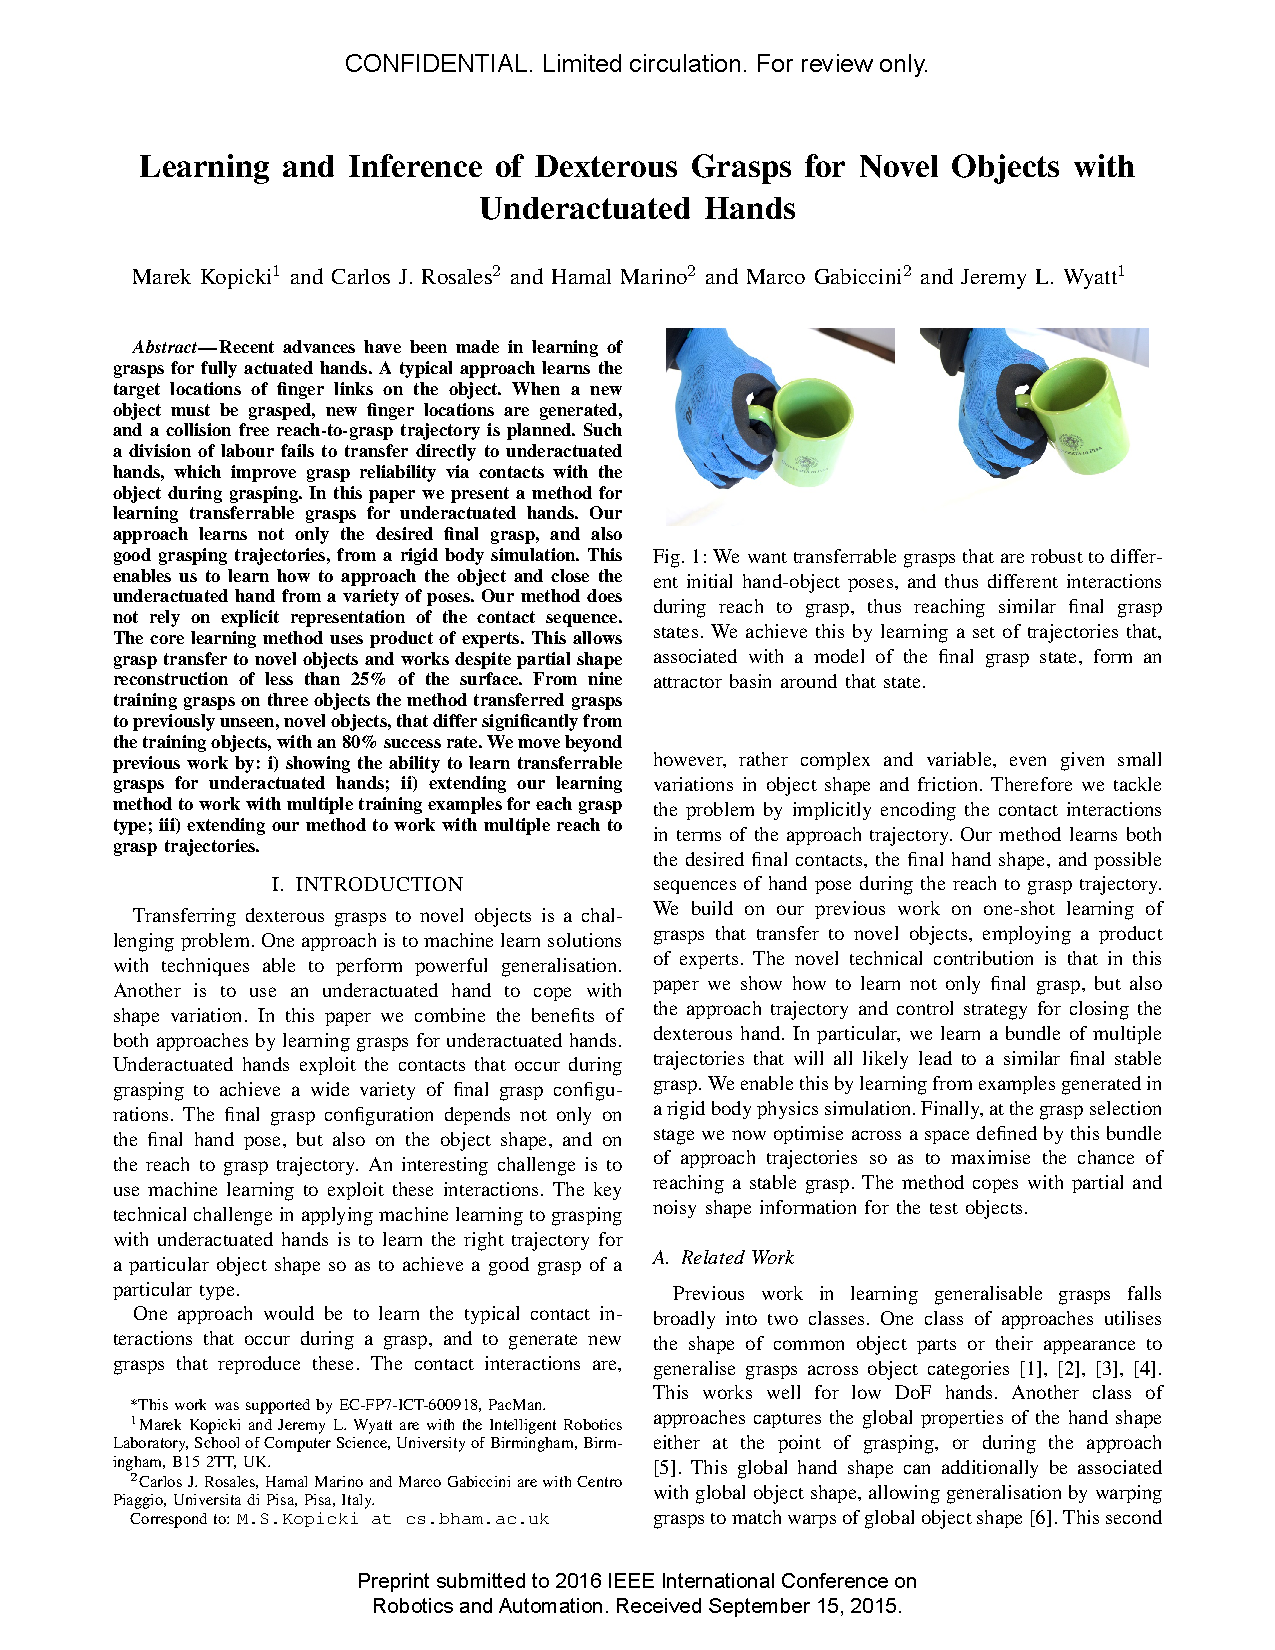
\includepdf[pages=-]{./attachedPapers/LearningInferenceUnderactuatedHands.pdf}

%%%%%%%%%%%%%%%%%%%%%%%%%%%%%%%%%%%%%%%%%%%%%%%%%%%%%%%%%%%%%%%%%%%%%%%%%%%%%%

\subsection{Article: Data-Driven Human Grasp Movement Analysis}
\label{ann:DataDrivenHumanGraspMovementAnalysis}
\begin{description}
    \item[Authors] H. Marino, M. Gabiccini, A. Leonardis, and A. Bicchi
    \item[Info] Submitted to: {\color{red} update this and the attached PDF!}
    \item[Abstract] The description of human hand motions is very complex, and methods to reduce this complexity have attracted much attention in the motor control literature. Important implications in robot hand design and programming have also generated a wide interest in the robotics research community.
    Early studies prevalently used direct analysis methods such as visual inspection to define grasp taxonomies. More recently, analytical methods have been employed to perform grasping data dimensionality reduction. In this paper, we present a methodology to reconcile these two distinct and apparently incompatible approaches under a unified framework: this allows us to obtain a data-generated grasp taxonomy along with low-dimensional representations which could be used for human grasping data classification and posture reconstruction, as well as for simplifying grasp planning algorithms and robotic hands programming.
%    Humans tend to simplify the space of possible grasps they can perform. This led to the introduction of grasp taxonomies via direct inspection of human movements, and data dimensionality reduction methods for grasp classification, robotic grasp synthesis, and simple hands design. In this paper, we present a methodology to reconcile these two distinct and apparently incompatible approaches under a unified framework, obtaining a data-driven taxonomy that can serve as a link among the aforementioned solutions.
    \item[Relation with the deliverable] this work is concerned with the problem of finding a principled way of analyzing human grasping motion in order to obtain guidelines for the design of hand underactuation mechanisms based on specific tasks to be accomplished.
    \item[Attachment] (following pages until next annex)
\end{description}
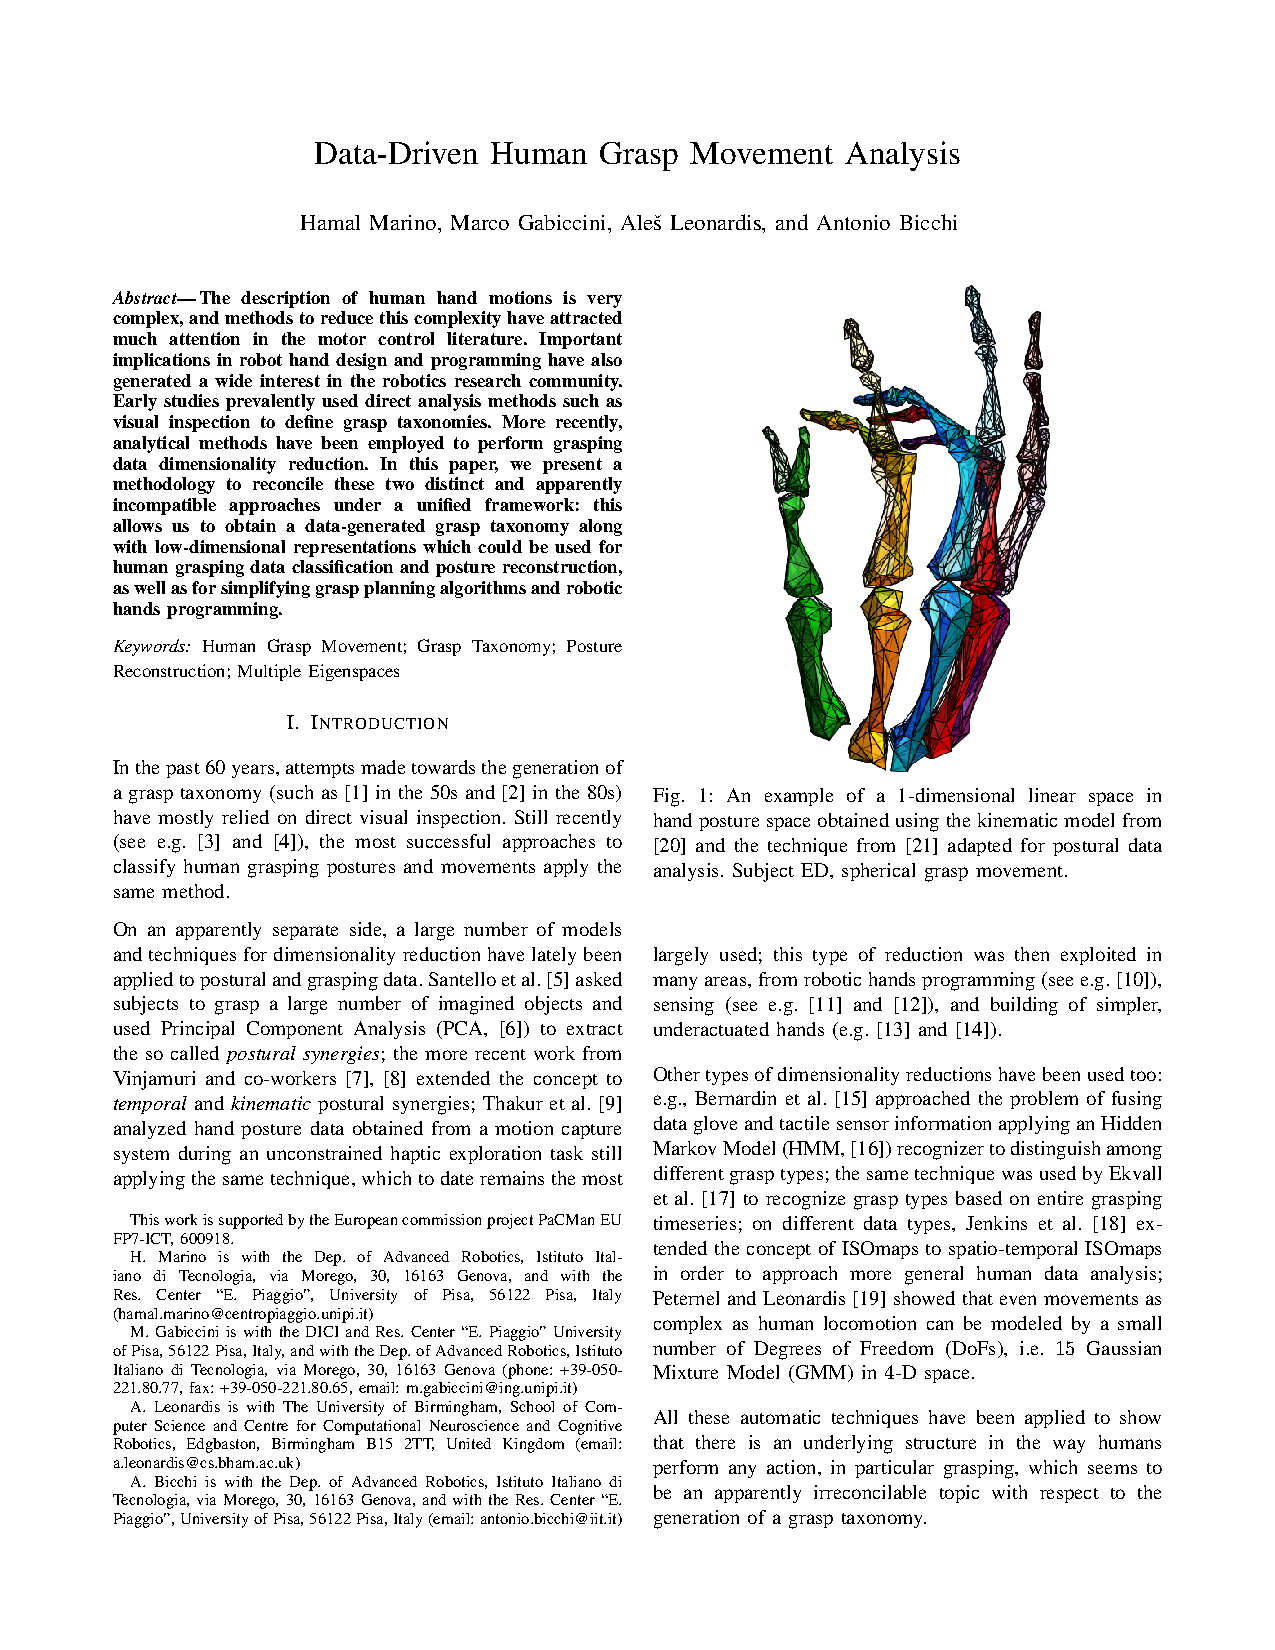
\includepdf[pages=-]{./attachedPapers/marino2015datadriven.pdf}

%%%%%%%%%%%%%%%%%%%%%%%%%%%%%%%%%%%%%%%%%%%%%%%%%%%%%%%%%%%%%%%%%%%%%%%%%%%%%%

\subsection{Article: A computational framework for environment-aware robotic manipulation planning} \label{ann:env-awareManipulation}
\begin{description}
    \item[Authors] M. Gabiccini, A. Artoni, G. Pannocchia, J.~Gillis
    \item[Info] Published in: 17th International Symposium on Robotics Research (ISRR), Sestri Levante (Genova), Italy, September 12-15, 2015
    \item[Abstract] In this paper, we present a computational framework for direct trajectory optimization of general manipulation systems with unspecified contact sequences, exploiting \emph{environmental constraints} as a key tool to accomplish a task.
    Two approaches are presented to describe the dynamics of systems with contacts, which are based on a penalty formulation and on a velocity-based time-stepping scheme, respectively. In  both cases, object and environment contact forces are included among the free optimization variables, and they are rendered consistent via suitably devised sets of complementarity conditions.
    To maximize computational efficiency, we exploit sparsity patterns in the linear algebra expressions generated during the solution of the optimization problem and leverage Algorithmic Differentiation to calculate derivatives. % quickly and accurately.
    The benefits of the proposed methods are evaluated in three simulated planar manipulation tasks, where essential interactions with environmental constraints are automatically synthesized and opportunistically exploited.
    \item[Relation with the deliverable] grasp and manipulation planning for systems with a-priori unspecified contact sequences.
    \item[Attachment] (following pages until next annex)
\end{description}
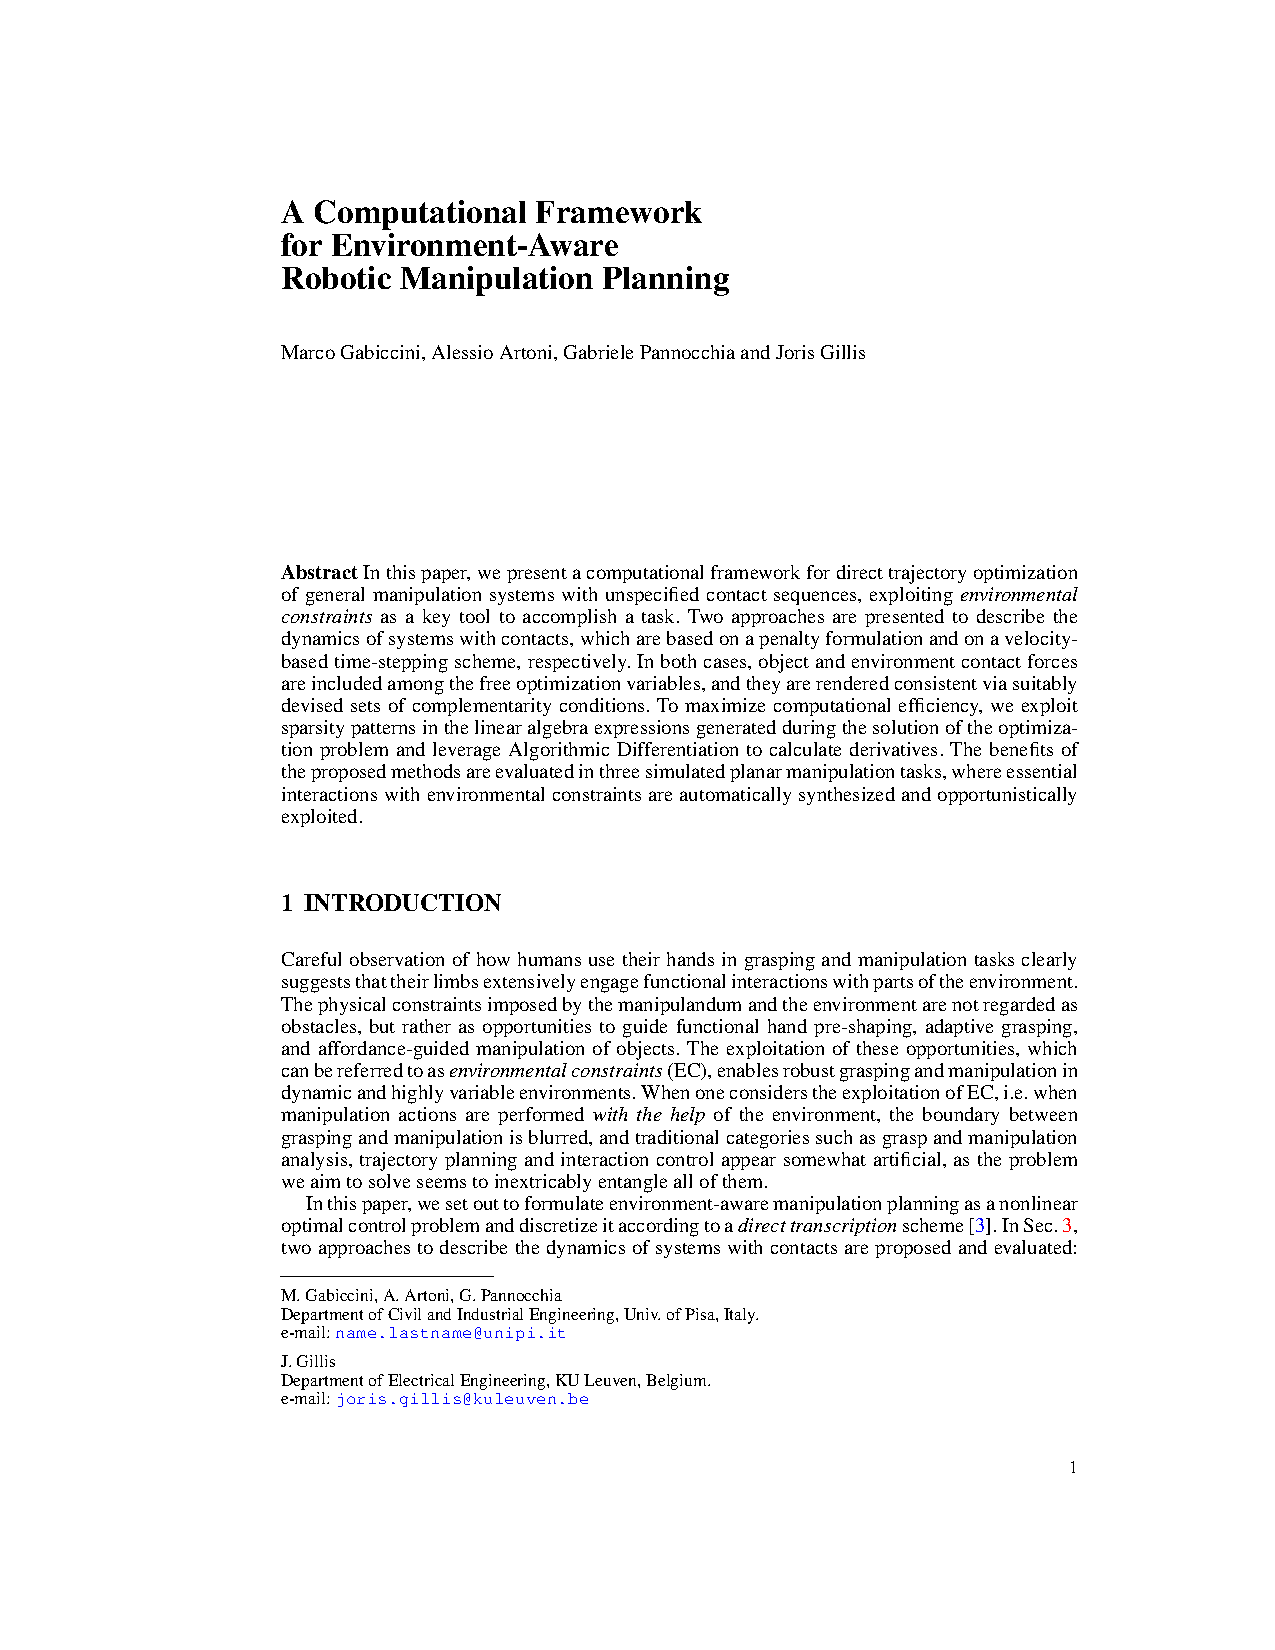
\includepdf[pages=-]{./attachedPapers/ComputationalFrameworkEnvAwareRobManipPlanning.pdf}
%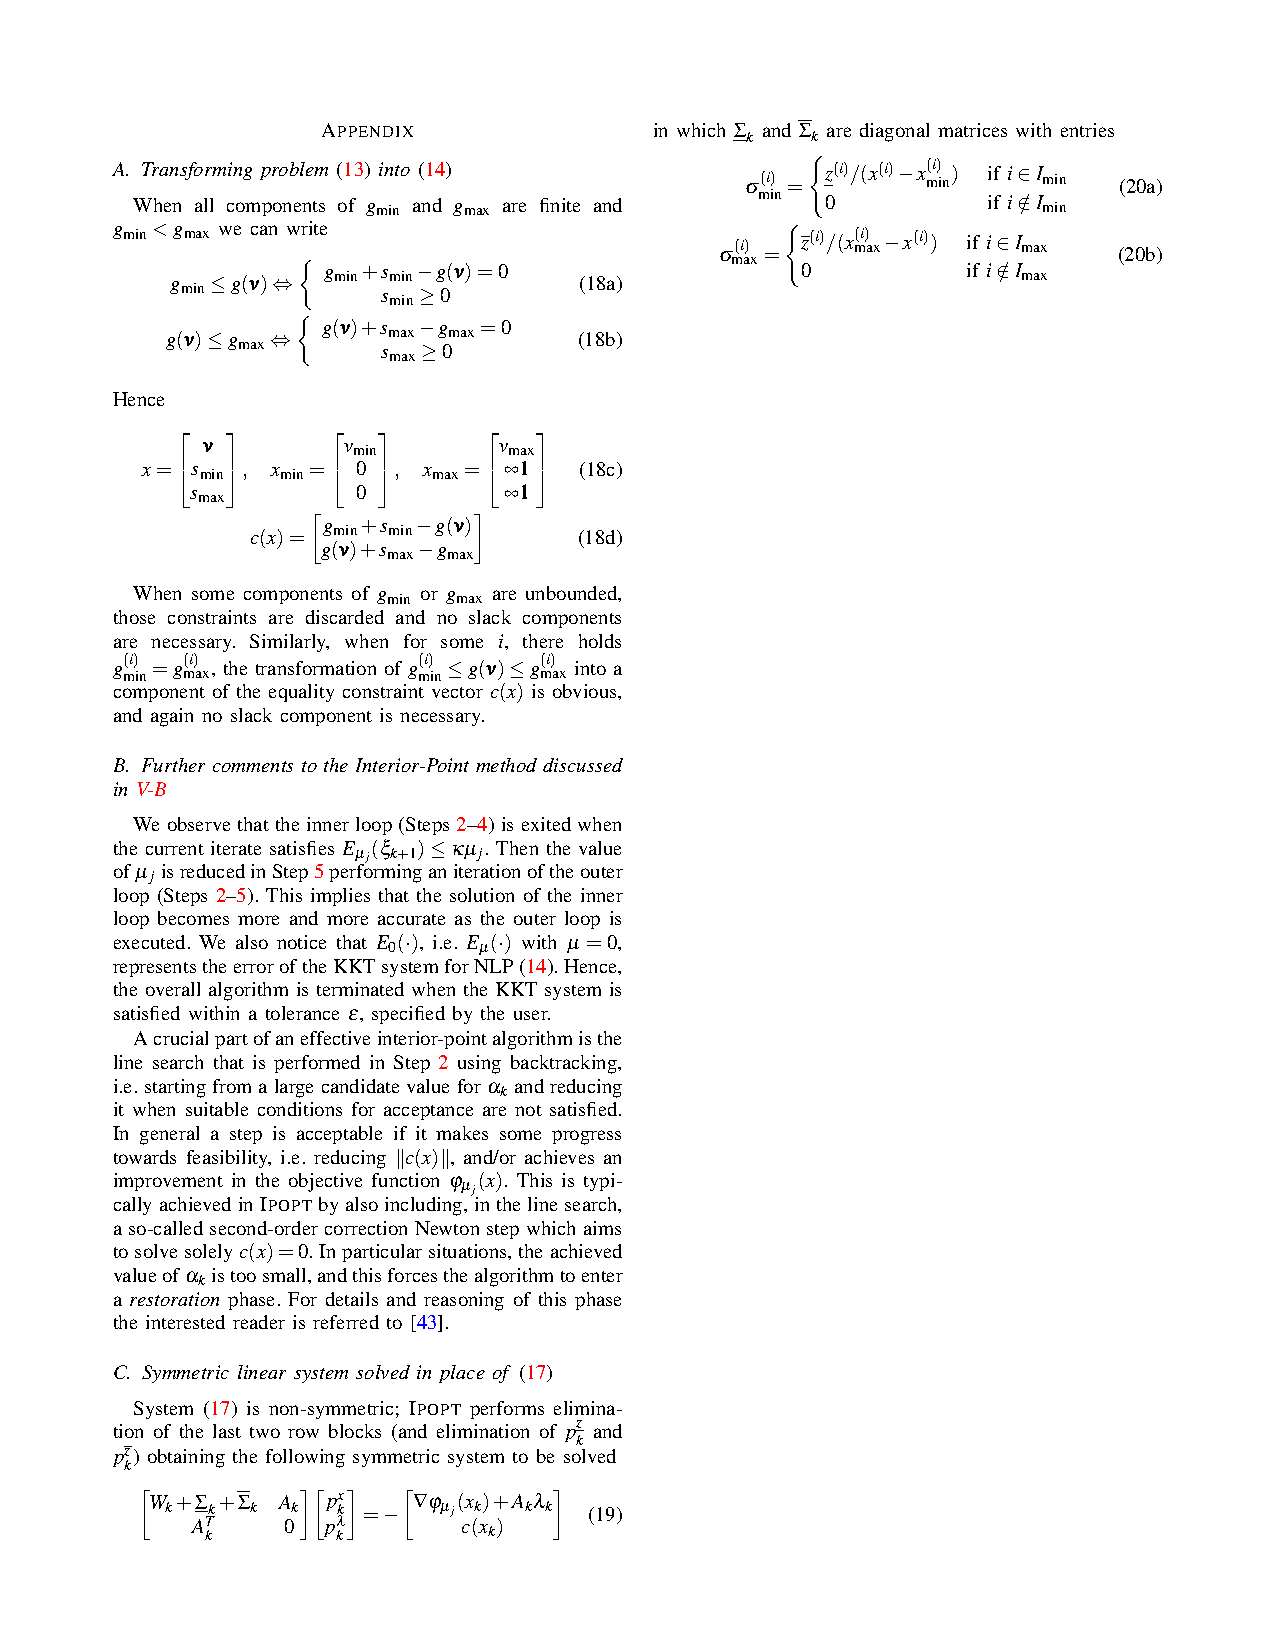
\includepdf[pages=-]{./attachedPapers/appendix_of_ComputationalFrameworkEnvAwareRobManipPlanning.pdf}

%%%%%%%%%%%%%%%%%%%%%%%%%%%%%%%%%%%%%%%%%%%%%%%%%%%%%%%%%%%%%%%%%%%%%%%%%%%%%%

\subsection{Article: Offset-free MPC explained: novelties, subtleties, and applications}
\label{ann:OffsetFreeMPCExplained}
\begin{description}
    \item[Authors] G. Pannocchia, M. Gabiccini, and A. Artoni
    \item[Info] Published in: 5th IFAC Conference on Nonlinear Model Predictive Control, Seville, Spain, September 17-20, 2015
    \item[Abstract]  This paper presents an updated and comprehensive description of offset-free MPC algorithms for nonlinear (and linear) discrete-time systems, with the intended objectives of clarifying the main concepts, showing new results, highlighting subtleties by means of challenging applications. First, the offset-free tracking problem for nonlinear systems is presented, putting a strong accent on the role of the disturbance model and observer, and then novel and stronger offset-free estimation results are presented. Next, recent advances in linear offset-free MPC are described, which show the equivalence of the velocity form algorithm (so far considered an alternative method) to a particular disturbance model and observer. Then, the concepts of offset-free estimation are exploited to design an offset-free economic MPC algorithm, which can asymptotically achieve the highest economic performance despite persistent model errors and disturbances. Extensive application results are presented to show the benefits of offset-free MPC algorithms over standard ones, and to clarify misconceptions and design errors that can prevent constraint satisfaction, closed-loop stability, and offset-free performance.
    \item[Relation with the deliverable] this work is concerned with providing the necessary theoretical background to design offset-free MPC algorithms, which are fundamental to turn direct trajectory optimization-based manipulation planners (presented in Sec.~\ref{sec:ComputationalFramework}) into controllers able to asymptotically achieve economic performances despite model errors and disturbances.
    \item[Attachment] (following pages until next annex)
\end{description}
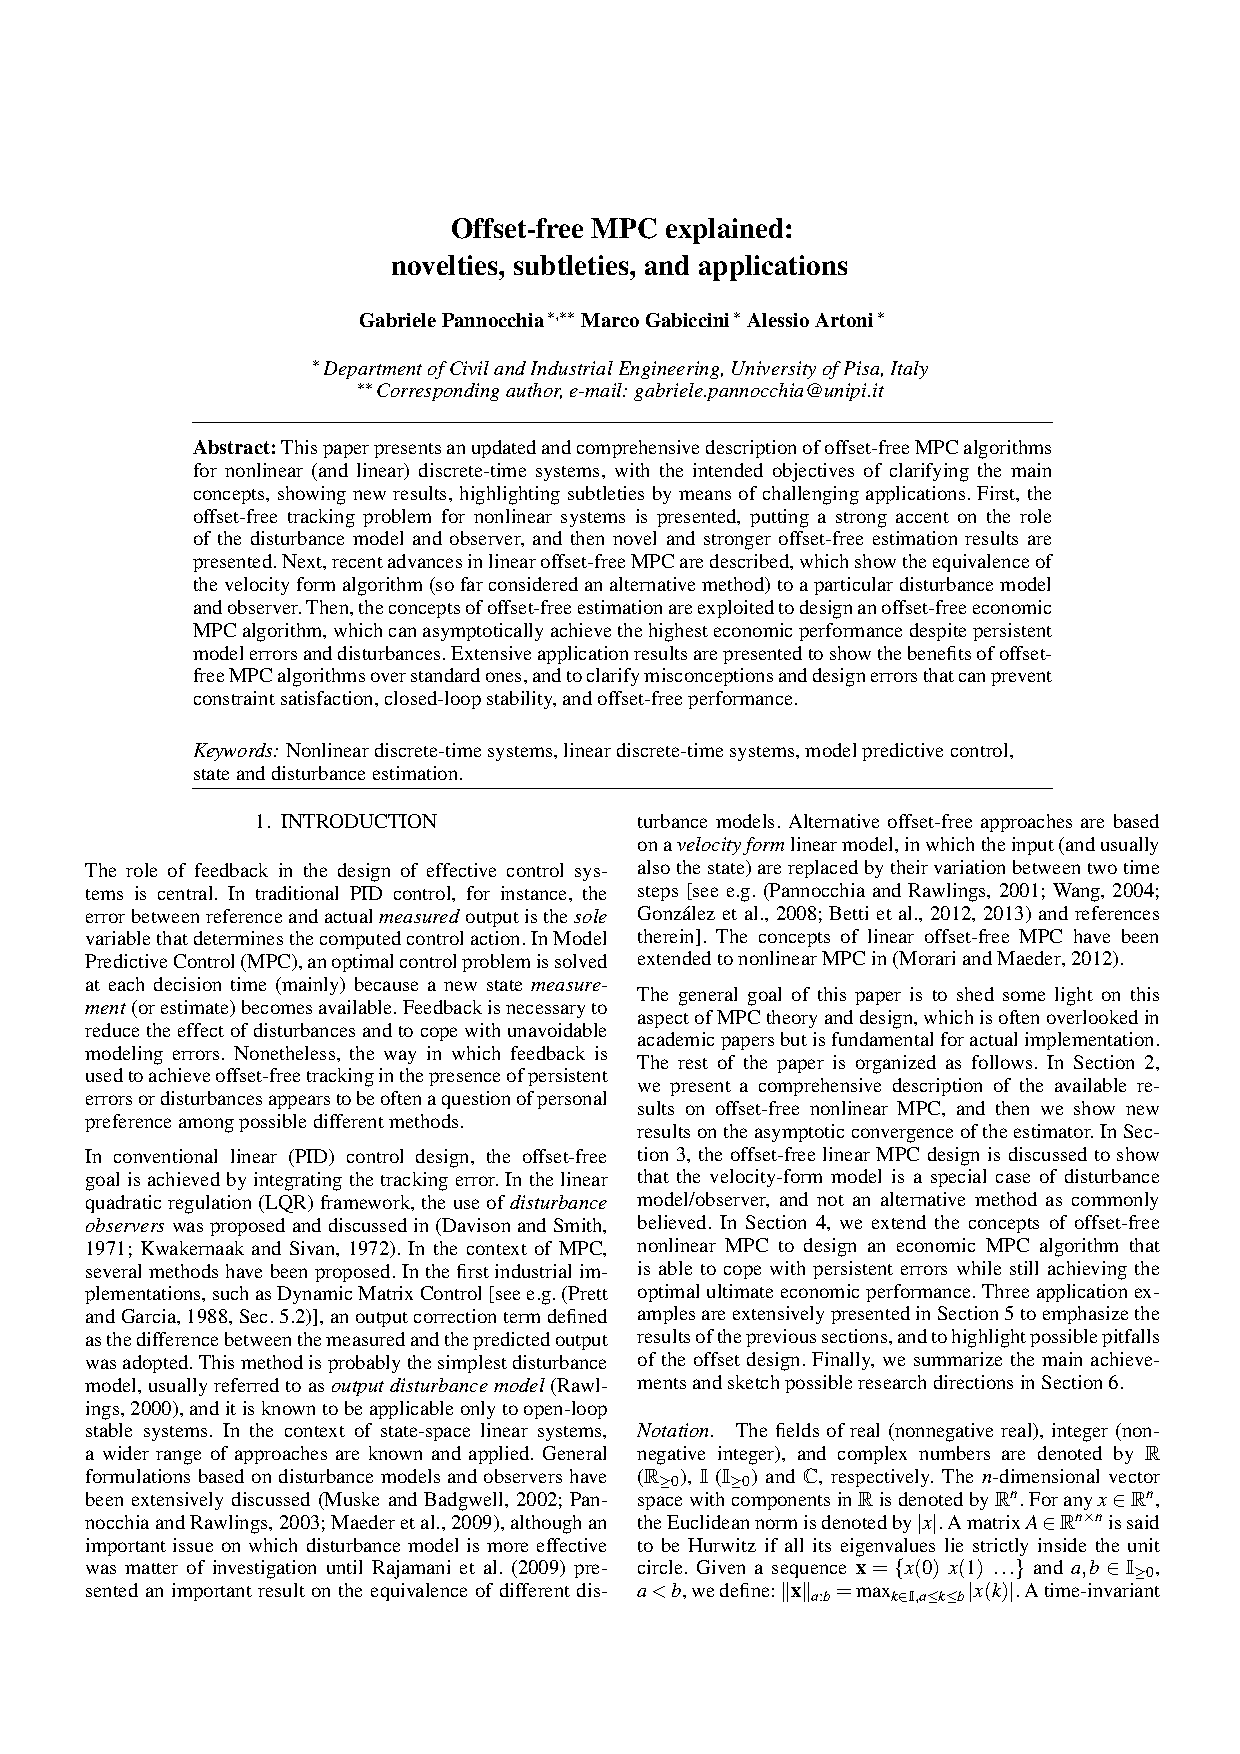
\includepdf[pages=-]{./attachedPapers/OffsetFreeMPCExplained.pdf}


\end{document}
